\chapter{費米子、狄拉克矩陣與狄拉克海}

狄拉克海是我們要探討的終點，但抵達的路徑也很重要。在處理相對論性電子理論中的負能量之前，我們需要先掌握兩項工具。首先是用來區分費米子與玻色子的算符代數；接著回顧一維狄拉克方程，藉此不必借助三維空間幾何，就能清楚看出波函數的每一次擴充。掌握這些之後，三維方程便會要求我們採用相應的矩陣結構；而開頭談到的費米子態填滿與空缺，則會再次成為理解正電子的關鍵。

我們採用\(c=\hbar=1\)。大寫\(P\)表示動量算符，小寫\(p\)表示動量本徵值，粗體符號則表示它們的三維版本。

\section{交換如何化為算符代數}

考慮兩個全同粒子，一個位於\(x\)，另一個位於\(y\)。標記\(x\)和\(y\)表示完整的位置，並非單一粒子的兩個笛卡兒座標。以兩個產生算符作用於真空，得到
\begin{equation}
\lvert x,y\rangle
=
\psi^\dagger(x)\psi^\dagger(y)\lvert0\rangle.
\label{eq:l10-two-particle-state}
\end{equation}

對玻色子而言，交換這兩個位置不會改變量子態：
\begin{equation}
\lvert x,y\rangle=\lvert y,x\rangle.
\end{equation}
確保這種對稱性的算符關係是
\begin{equation}
\psi^\dagger(x)\psi^\dagger(y)
=
\psi^\dagger(y)\psi^\dagger(x).
\label{eq:l10-boson-exchange}
\end{equation}
兩個玻色子產生算符彼此對易，因此交換它們的順序，不會改變所產生的量子態。

對費米子而言，交換會使符號反轉：
\begin{equation}
\lvert x,y\rangle=-\lvert y,x\rangle.
\label{eq:l10-fermion-state-exchange}
\end{equation}
單一態向量的整體符號無法觀測，但不同可能性之間的相對符號可以觀測，因此必須一致地保留這個負號。式~\eqref{eq:l10-fermion-state-exchange}要求
\begin{equation}
\psi^\dagger(x)\psi^\dagger(y)
=
-\,\psi^\dagger(y)\psi^\dagger(x).
\label{eq:l10-fermion-operator-exchange}
\end{equation}

\begin{figure}[htbp]
\centering
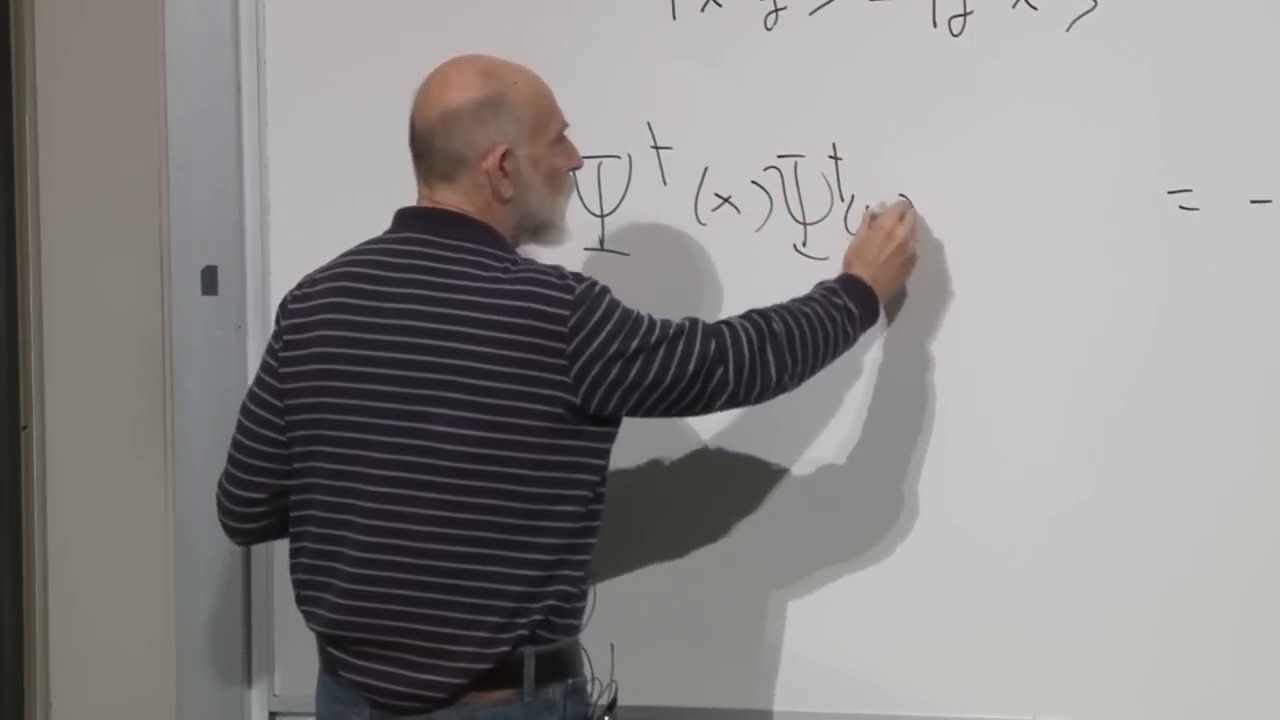
\includegraphics[width=0.94\linewidth]{lecture_10_figure_02.png}
\caption{黑板上表示費米子交換的關係。交換產生算符的順序，會使兩粒子態的符號反轉。}
\lectureframe{00:05:50}
\end{figure}

對任意兩個算符\(A\)和\(B\)，反對易子定義為
\begin{equation}
\{A,B\}:=AB+BA.
\end{equation}
因此，交換規則是
\begin{equation}
\{\psi^\dagger(x),\psi^\dagger(y)\}=0.
\label{eq:l10-creation-anticommutator}
\end{equation}
相應的費米子場代數以反對易子取代玻色子場的對易子。這裡必須區分「反對易」一詞的兩種用法：場算符因費米統計而反對易；稍後矩陣彼此反對易，則是為了消去相對論性色散關係中的交叉項。

現在在式~\eqref{eq:l10-creation-anticommutator}中令\(y=x\)。兩個乘積便相同：
\begin{align}
0
&=\{\psi^\dagger(x),\psi^\dagger(x)\}\\
&=2\,\psi^\dagger(x)\psi^\dagger(x).
\end{align}
因此
\begin{equation}
\bigl(\psi^\dagger(x)\bigr)^2=0.
\label{eq:l10-exclusion}
\end{equation}
若試圖在同一單粒子態中產生兩個相同的費米子，結果會是零向量。這就是排他原理的算符形式。

\begin{figure}[htbp]
\centering
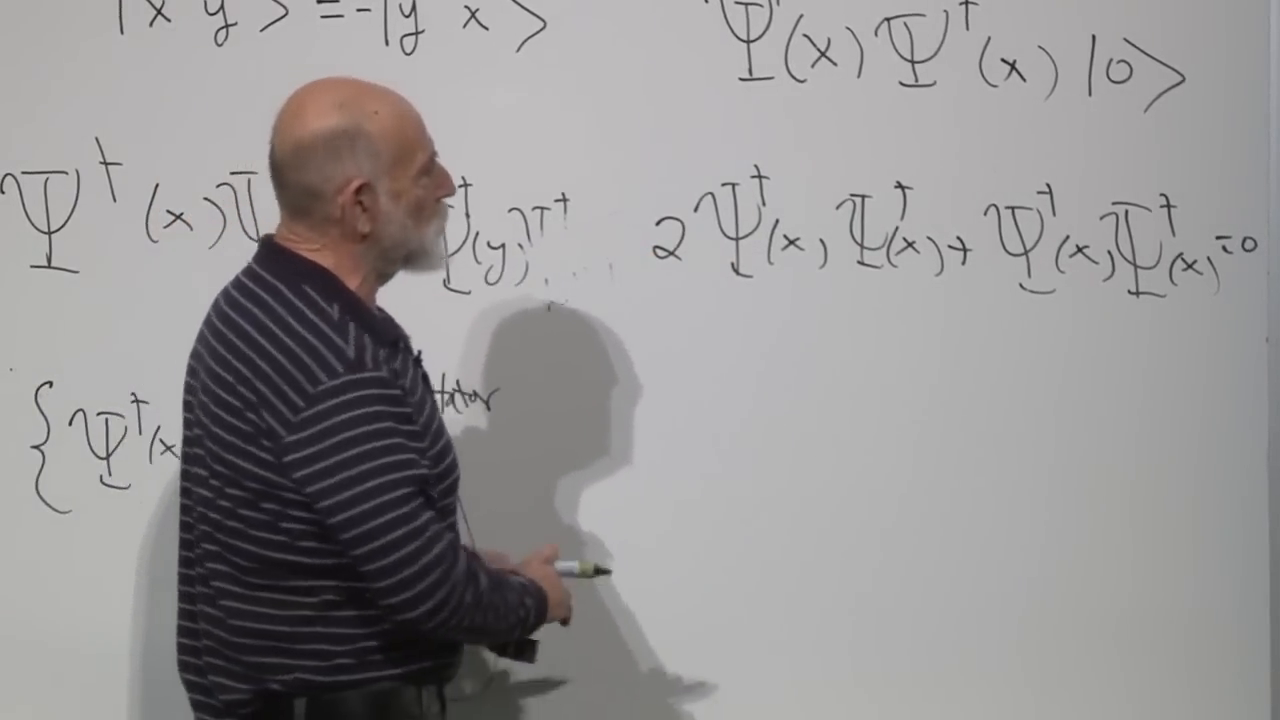
\includegraphics[width=0.94\linewidth]{lecture_10_figure_03.png}
\caption{黑板上將兩態取為相同態的情形。重複的產生算符乘積出現兩次，因此必須為零。}
\lectureframe{00:08:04}
\end{figure}

\begin{figure}[htbp]
\centering
\begin{adjustbox}{max width=\linewidth}
\begin{tikzpicture}[node distance=1.25cm,>=Latex]
\node[draw,rounded corners,align=center,inner sep=7pt] (a)
  {$\{\psi^\dagger(x),\psi^\dagger(x)\}=0$};
\node[draw,rounded corners,align=center,inner sep=7pt,right=of a] (b)
  {$2(\psi^\dagger(x))^2=0$};
\node[draw,rounded corners,align=center,inner sep=7pt,right=of b] (c)
  {$(\psi^\dagger(x))^2=0$};
\draw[->,thick] (a) -- (b);
\draw[->,thick] (b) -- (c);
\end{tikzpicture}
\end{adjustbox}
\caption{不依賴黑板上已部分擦除的中間推導，重新呈現排他原理的論證。}
\end{figure}

\section{為什麼費米子的填滿態與空態具有對稱性}

玻色子與費米子算符之間還有第二個差異，這個差異比排他原理更微妙，對後續內容也至關重要。對單一玻色子模態而言，
\begin{equation}
[a,a^\dagger]=1,
\qquad
n=0,1,2,\ldots.
\end{equation}
交換\(a\)與\(a^\dagger\)，會使對易子的符號反轉。即使只把這些算符稱作\(A\)和\(B\)，代數仍會指出哪種排列會增加佔據數，哪種會減少佔據數。

玻色子的佔據階梯也有方向。湮滅算符最終會到達\(\lvert0\rangle\)，並將它化為零；產生算符則可以不斷繼續作用：
\begin{align}
a\lvert0\rangle&=0,\\
a^\dagger\lvert n\rangle&\propto\lvert n+1\rangle,
\qquad n=0,1,2,\ldots.
\end{align}
將這個階梯上下顛倒，並不會得到相同的能譜。它有底端，卻沒有頂端。

對單一費米子模態而言，
\begin{equation}
\{a,a^\dagger\}=1,
\qquad
a^2=(a^\dagger)^2=0,
\qquad
n=0,1.
\label{eq:l10-fermion-mode}
\end{equation}
產生算符將空態變為滿態，之後便停止作用：
\begin{equation}
a^\dagger\lvert0\rangle=\lvert1\rangle,
\qquad
a^\dagger\lvert1\rangle=0.
\end{equation}
湮滅算符則執行相反的操作：
\begin{equation}
a\lvert1\rangle=\lvert0\rangle,
\qquad
a\lvert0\rangle=0.
\end{equation}
只有兩種態，因此交換滿態與空態，並交換\(a\)與\(a^\dagger\)，圖示仍保持對稱。這兩個算符的物理意義仍然不同，但它們的代數不再特別指定其中一個為產生算符、另一個為湮滅算符。這種形式上的對稱性，正是粒子—空穴重新詮釋的起點。

\begin{classroomqa}
\lecturetimestamp{00:13:54}
\audiencequestion{如果\((a^\dagger)^2=0\)，這是矛盾嗎？還是表示\(a^\dagger=0\)？}
\lecturerresponse{兩者皆非。非零算符的平方可以為零。這裡，\(a^\dagger\)將\(\lvert0\rangle\)變為\(\lvert1\rangle\)，但\(\lvert1\rangle\)之上沒有可允許的態，因此對它作用兩次，結果為零。同理可得\(a^2=0\)。}
\end{classroomqa}

先記住這種滿態與空態之間的對稱性。移除一個負能量電子時，湮滅算符會重新標記為正電子產生算符。這不是任意更改符號，而是運用了此處建立的兩態費米子代數。

\section{一維狄拉克方程的構造}

現在回到一維空間中的單一粒子。最簡單的一階相對論性波動方程是
\begin{equation}
i\partial_t\psi=-\,i\partial_x\psi.
\label{eq:l10-right-mover}
\end{equation}
取\(P=-i\partial_x\)後，方程成為
\begin{equation}
H=P.
\end{equation}
動量本徵態滿足\(E=p\)，其群速度為
\begin{equation}
v_g=\frac{dE}{dp}=1.
\end{equation}
動量為正或為負，因而能量為正或為負，波仍都以固定形狀向右傳播。\(p\)的符號會改變相位的分布，而非傳播方向。

有質量的粒子必須能向任一方向運動。引入第二個分量，使其滿足
\begin{equation}
H\psi_1=P\psi_1,
\qquad
H\psi_2=-P\psi_2.
\label{eq:l10-two-directions}
\end{equation}
第一個分量向右傳播，第二個分量向左傳播。將兩者排成一個欄向量，
\begin{equation}
\Psi=
\begin{pmatrix}
\psi_1\\
\psi_2
\end{pmatrix},
\end{equation}
並定義
\begin{equation}
\alpha=
\begin{pmatrix}
1&0\\
0&-1
\end{pmatrix}.
\end{equation}
兩個方程便都可以寫成
\begin{equation}
H\Psi=\alpha P\Psi.
\label{eq:l10-massless-one-d}
\end{equation}
納入兩個傳播方向，代價是引入一個新的二值內部自由度。

只有傳播方向還不足以產生質量。引入第二個矩陣，
\begin{equation}
\beta=
\begin{pmatrix}
0&1\\
1&0
\end{pmatrix},
\end{equation}
並令哈密頓量為
\begin{equation}
H=\alpha P+\beta m.
\label{eq:l10-massive-one-d}
\end{equation}
這些矩陣滿足
\begin{equation}
\alpha^2=\beta^2=\mathbb{1},
\qquad
\{\alpha,\beta\}=0.
\label{eq:l10-one-d-algebra}
\end{equation}
將哈密頓量平方，得到
\begin{align}
H^2
&=(\alpha P+\beta m)^2\\
&=\alpha^2P^2+\beta^2m^2
  +(\alpha\beta+\beta\alpha)Pm\\
&=P^2+m^2.
\label{eq:l10-one-d-dispersion}
\end{align}
式~\eqref{eq:l10-one-d-algebra}中的反對易子會消去同時含有\(P\)與\(m\)的多餘項。

非對角矩陣\(\beta\)將兩個方向分量耦合起來。可以把質量項想成持續混合向右與向左傳播的振幅。這個圖像不應被理解成粒子真的沿著微觀軌道來回彈跳，但它說明了為何有質量波包的平均速度可以低於光速，也說明了為何它可以有靜止參考系，而孤立的無質量手徵分量則不能。

\begin{classroomqa}
\lecturetimestamp{00:23:37}
\audiencequestion{引入兩個方向分量，是否有更深一層的物理解釋？}
\lecturerresponse{有，不過到了三維時，這種解釋會更清楚。目前這兩個分量只是描述相反傳播方向、並容許非對角質量耦合所必需的分量。它們後來會被詮釋為左右手性，也就是相反的手徵性。}
\end{classroomqa}

\section{三維空間要求泡利矩陣}

在三維空間中，動量是向量。若哈密頓量對動量呈線性且為旋轉標量，自然會引入另一個向量；這次它的分量是矩陣：
\begin{equation}
H=\boldsymbol{\alpha}\cdot\mathbf P
=\alpha_xP_x+\alpha_yP_y+\alpha_zP_z.
\label{eq:l10-three-d-ansatz}
\end{equation}

\begin{figure}[htbp]
\centering
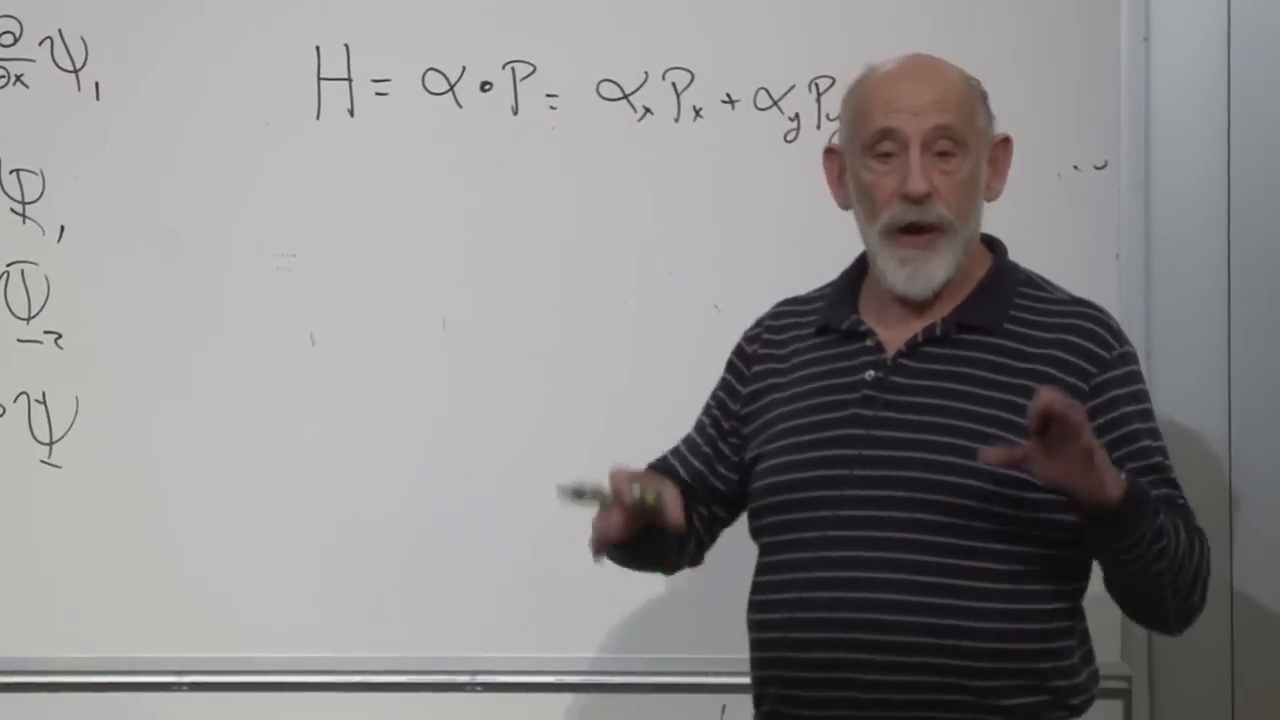
\includegraphics[width=0.94\linewidth]{lecture_10_figure_04.png}
\caption{三維無質量假設\(H=\boldsymbol{\alpha}\cdot\mathbf P\)，圖中正顯示一個矩陣如何成為由三個矩陣組成的向量。}
\lectureframe{00:26:00}
\end{figure}

再次從無質量情形開始。我們要求
\begin{equation}
H^2=\mathbf P^2=P_x^2+P_y^2+P_z^2.
\end{equation}
將式~\eqref{eq:l10-three-d-ansatz}平方後展開，得到
\begin{align}
H^2
&=\alpha_x^2P_x^2+\alpha_y^2P_y^2\\
&\quad+\alpha_z^2P_z^2\\
&\quad+\{\alpha_x,\alpha_y\}P_xP_y\\
&\quad+\{\alpha_x,\alpha_z\}P_xP_z\\
&\quad+\{\alpha_y,\alpha_z\}P_yP_z.
\end{align}
若滿足
\begin{equation}
\alpha_x^2=\alpha_y^2=\alpha_z^2=\mathbb{1},
\end{equation}
對角項就會正確；若滿足
\begin{equation}
\{\alpha_i,\alpha_j\}=0,
\qquad i\ne j.
\label{eq:l10-alpha-anticommutation}
\end{equation}
所有交叉項便會消失。

三個熟知的\(2\times2\)矩陣恰好符合這些要求：
\begin{equation}
\sigma_x=
\begin{pmatrix}
0&1\\
1&0
\end{pmatrix},
\quad
\sigma_y=
\begin{pmatrix}
0&-i\\
i&0
\end{pmatrix},
\quad
\sigma_z=
\begin{pmatrix}
1&0\\
0&-1
\end{pmatrix}.
\label{eq:l10-pauli-matrices}
\end{equation}
因此，一個解為
\begin{equation}
\alpha_i=\sigma_i,
\qquad
H=\boldsymbol{\sigma}\cdot\mathbf P.
\label{eq:l10-weyl-hamiltonian}
\end{equation}

\begin{figure}[htbp]
\centering
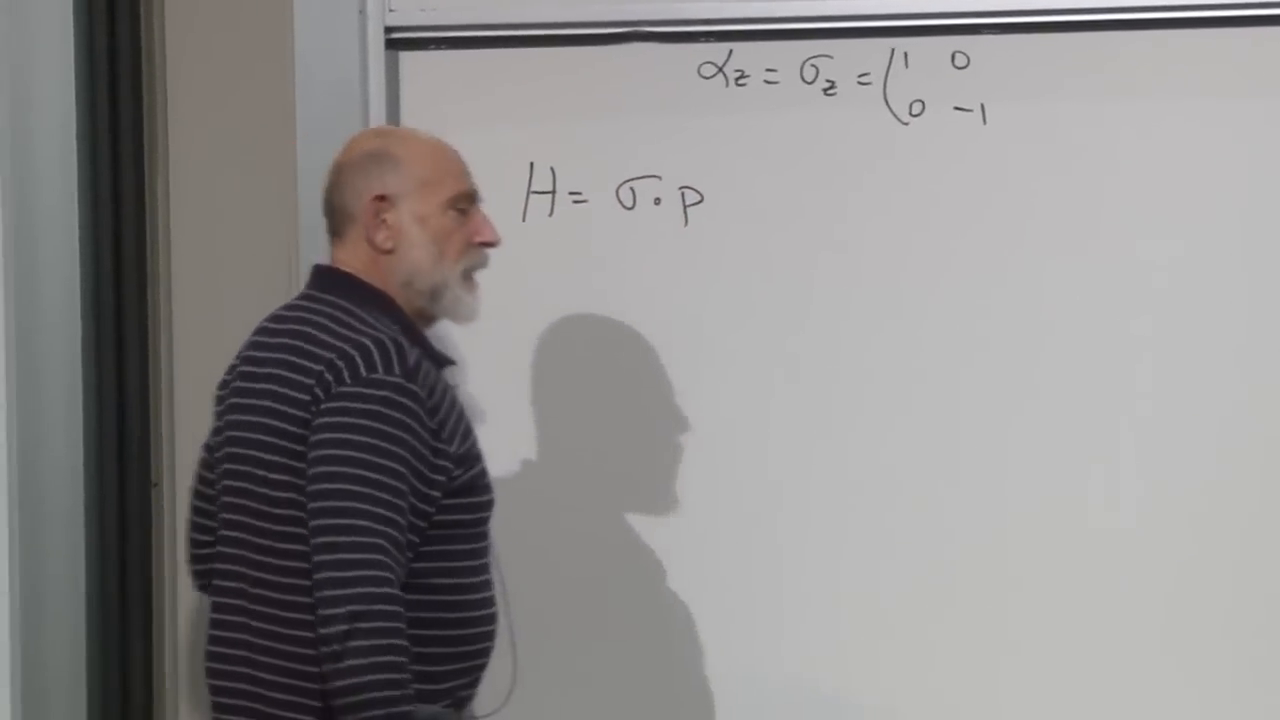
\includegraphics[width=0.94\linewidth]{lecture_10_figure_05.png}
\caption{緊湊的無質量哈密頓量\(H=\boldsymbol{\sigma}\cdot\mathbf P\)；上方仍可看到\(\alpha_z=\sigma_z\)。}
\lectureframe{00:28:16}
\end{figure}

對動量本徵態而言，
\begin{equation}
\boldsymbol{\sigma}\cdot\mathbf p
=
|\mathbf p|\,\boldsymbol{\sigma}\cdot\widehat{\mathbf p}.
\end{equation}
算符\(\boldsymbol{\sigma}\cdot\widehat{\mathbf p}\)的本徵值為\(+1\)和\(-1\)，因此
\begin{equation}
E=\pm|\mathbf p|.
\end{equation}
在這個二分量理論中，正能態的泡利自由度與動量同向，負能態則與動量反向。這種對齊關係是固定的；能量符號給定後，自旋方向不能再獨立調整。

\begin{classroomqa}
\lecturetimestamp{00:30:10}
\audiencequestion{自旋是從狄拉克方程推導出來的，還是因為已知電子具有磁矩，才把自旋放進方程？}
\lecturerresponse{這裡「推導出來」的意思是「作為結果出現」，不是「消失」。我們一開始要求哈密頓量對動量呈線性，且其平方為\(\mathbf P^2\)。普通數無法滿足所需的代數關係，但泡利矩陣可以。因此，線性化本身便帶入了二分量結構。這並不證明每種粒子都必須具有自旋；它表示，以這類狄拉克方程描述的粒子，具有相應的旋量自由度。}
\end{classroomqa}

這是此一構造的核心教訓之一。矩陣不是找到相對論性方程之後才加上的裝飾標記；試圖對相對論性色散關係取局域平方根，便會導出這些矩陣。

\section{為什麼質量需要四個分量}

試著不擴充\(2\times2\)理論，重做一維情形中引入質量的構造：
\begin{equation}
H=\boldsymbol{\sigma}\cdot\mathbf P+\beta m.
\label{eq:l10-failed-mass}
\end{equation}
假設\(\beta^2=\mathbb{1}\)。平方後會出現所需的項\(\mathbf P^2+m^2\)，但也會出現
\begin{equation}
m\sum_i\{\sigma_i,\beta\}P_i.
\end{equation}
若要消去這一項，矩陣\(\beta\)必須滿足
\begin{equation}
\{\sigma_x,\beta\}
=
\{\sigma_y,\beta\}
=
\{\sigma_z,\beta\}
=0.
\label{eq:l10-impossible-beta}
\end{equation}
然而不存在符合要求的\(2\times2\)矩陣。單位矩陣與所有三個泡利矩陣對易，而任何無跡的\(2\times2\)矩陣都是泡利矩陣的線性組合。這類組合都無法與平行於它的分量反對易。\(2\times2\)代數中不存在符合要求的第四個獨立矩陣。

解決方法是擴充旋量。四個彼此反對易且平方為單位矩陣的矩陣，最早可在\(4\times4\)複數表示中實現。選擇這種矩陣大小，不是因為時空有四個維度，而是因為這是能實現所需代數的最小矩陣空間。

等價表示有很多種。對旋量基底作么正變換，會改變所有矩陣的元素，但不會改變任何物理預測。重要的是以下這組抽象關係：
\begin{equation}
\{\alpha_i,\alpha_j\}=2\delta_{ij}\mathbb{1},
\qquad
\{\alpha_i,\beta\}=0,
\qquad
\beta^2=\mathbb{1}.
\label{eq:l10-dirac-algebra}
\end{equation}

\begin{classroomqa}
\lecturetimestamp{00:37:38}
\audiencequestion{能否將\(\beta\)視為時間分量\(\alpha_t\)？}
\lecturerresponse{不能直接這麼看。三個\(\alpha_i\)與\(\beta\)並不會合成單一洛倫茲向量的四個分量。在協變記號中，我們改為定義\(\beta=\gamma^0\)與\(\alpha_i=\gamma^0\gamma^i\)；四個\(\gamma^\mu\)矩陣則滿足時空克利福德代數。}
\end{classroomqa}

一種方便的分塊表示是
\begin{equation}
\alpha_i=
\begin{pmatrix}
\sigma_i&0\\
0&-\sigma_i
\end{pmatrix},
\qquad
\beta=
\begin{pmatrix}
0&I_2\\
I_2&0
\end{pmatrix}.
\label{eq:l10-block-representation}
\end{equation}
對角區塊中的泡利矩陣確保不同的\(\alpha_i\)彼此反對易。\(\beta\)中的非對角單位矩陣區塊則確保\(\beta\)與每個\(\alpha_i\)反對易。

\begin{figure}[htbp]
\centering
\includegraphics[width=0.94\linewidth]{lecture_10_figure_06.png}
\caption{黑板上的\(4\times4\)分塊表示。上方的方程列出所需的反對易關係；完整矩陣則列於式~\eqref{eq:l10-block-representation}。}
\lectureframe{00:41:10}
\end{figure}

有質量的哈密頓量現在為
\begin{equation}
H=\boldsymbol{\alpha}\cdot\mathbf P+\beta m
=
\begin{pmatrix}
\boldsymbol{\sigma}\cdot\mathbf P&mI_2\\
mI_2&-\boldsymbol{\sigma}\cdot\mathbf P
\end{pmatrix}.
\label{eq:l10-massive-dirac}
\end{equation}
利用式~\eqref{eq:l10-dirac-algebra}，可得
\begin{equation}
H^2=\mathbf P^2+m^2.
\end{equation}
因此，四分量結構並非可有可無的修飾；它是在保持方程為一階的同時，容納三維動量與質量項所需的最小結構。

\section{手徵性與額外分量的意義}

擴充旋量後，多出了什麼物理區別？先看無質量的上方區塊，
\begin{equation}
H_R=\boldsymbol{\sigma}\cdot\mathbf P,
\end{equation}
再看無質量的下方區塊，
\begin{equation}
H_L=-\boldsymbol{\sigma}\cdot\mathbf P.
\end{equation}
對正能態而言，第一個區塊的自旋與動量同向，第二個區塊的自旋與動量反向。兩者具有相反的螺旋度。在無質量理論中，螺旋度在正洛倫茲變換下保持不變，因為沒有觀察者能超越類光粒子、反轉其動量，同時維持其自旋方向不變。因此，這兩個區塊描述相反的手徵扇區。

\begin{classroomqa}
\lecturetimestamp{00:41:28}
\audiencequestion{一維情形中，引入質量需要額外的二值自由度。三維情形中，對應的物理區別是什麼？}
\lecturerresponse{是旋量的手徵性。兩個\(2\times2\)區塊中的自旋與動量具有相反的關係：一個是右手性，另一個是左手性。\(4\times4\)理論包含兩者。}
\end{classroomqa}

式~\eqref{eq:l10-massive-dirac}中的質量項是非對角的。它將上方區塊的振幅耦合到下方區塊，反之亦然：
\begin{equation}
\beta m
\begin{pmatrix}
\Psi_R\\
\Psi_L
\end{pmatrix}
=
m
\begin{pmatrix}
\Psi_L\\
\Psi_R
\end{pmatrix}.
\end{equation}
因此，質量會耦合相反手徵性的態。

\begin{classroomqa}
\lecturetimestamp{00:43:58}
\audiencequestion{無質量粒子能改變手徵性嗎？}
\lecturerresponse{在此處顯示的自由無質量哈密頓量中不能。兩個區塊彼此解耦，因此一個起初為右手性或左手性的態會維持原狀。當\(m\ne0\)時，非對角質量項正是混合兩者的原因。}
\end{classroomqa}

對分塊表示而言，這種說法是精確的；但不宜把粒子在兩個箭頭之間機械翻轉的圖像過度延伸。真正的物理敘述，是波動方程中的矩陣耦合。

\begin{classroomqa}
\lecturetimestamp{00:44:50}
\audiencequestion{這些矩陣是由四元數構成的嗎？}
\lecturerresponse{泡利矩陣與四元數單位密切相關：矩陣\(-i\sigma_i\)的平方為\(-\mathbb{1}\)，其乘法也符合四元數的形式，只有方向慣例上的差異。完整的狄拉克矩陣需要更大的克利福德代數，而接下來的論證不需要用到四元數的關聯。}
\end{classroomqa}

\begin{classroomqa}
\lecturetimestamp{00:46:34}
\audiencequestion{若自旋是角動量，這裡是否還有與自旋相關的獨立能量項？}
\lecturerresponse{沒有加入獨立的自由粒子項。旋量結構已透過矩陣納入動能哈密頓量。若將自旋與外加磁場耦合，會引入額外的交互作用項，但那是另一個問題。}
\end{classroomqa}

\section{{\proseunicodefont α}矩陣代表速度，不是自旋}

每個\(\alpha_i\)都有兩個\(+1\)本徵值，也有兩個\(-1\)本徵值。不同分量彼此不對易，因此無法同時精確測量。若要辨明其中一個分量代表什麼，可以使用海森堡方程。對於沒有顯式時間依賴的算符\(L\)，
\begin{equation}
\dot L=i[H,L].
\label{eq:l10-heisenberg}
\end{equation}
此處的符號慣例由Schr\"odinger演化\(e^{-iHt}\)決定。

將式~\eqref{eq:l10-heisenberg}用於位置算符\(x\)。這些矩陣作用於旋量指標，與位置算符對易；只有\(P_x\)不與\(x\)對易：
\begin{align}
\dot x
&=i[\boldsymbol{\alpha}\cdot\mathbf P+\beta m,x]\\
&=i\alpha_x[P_x,x]\\
&=\alpha_x,
\label{eq:l10-velocity}
\end{align}
因為\([P_x,x]=-i\)。因此，\(\alpha_x\)就是速度算符的\(x\)分量；同理，
\begin{equation}
\dot{\mathbf x}=\boldsymbol{\alpha}.
\end{equation}

\begin{classroomqa}
\lecturetimestamp{00:51:50}
\audiencequestion{速度分量的測量結果真的只有\(+1\)或\(-1\)嗎？}
\lecturerresponse{是的。以\(\alpha_i\)為瞬時算符，並採用\(c=1\)單位制時，結果確實如此。一般態不一定是本徵態，因此其期望值可以介於這兩個值之間。有質量粒子的波包平滑傳播，其平均速度低於光速。}
\end{classroomqa}

速度並非守恆量：
\begin{equation}
\dot\alpha_x=i[H,\alpha_x]\ne0.
\end{equation}
含有\(\alpha_y\)、\(\alpha_z\)和\(\beta\)的項都不與\(\alpha_x\)對易。因此，同時含有正能與負能分量的態，其位置會呈現快速振盪的部分。這就是\emph{zitterbewegung}，字面意思是顫動運動。

對遠長於快速振盪週期的時間取平均後，預期的相對論速度為
\begin{equation}
\overline{\mathbf v}=\frac{\mathbf p}{E},
\end{equation}
對低速電子而言，這會化為\(\mathbf p/m\)。

\begin{classroomqa}
\lecturetimestamp{00:54:40}
\audiencequestion{自由電子沒有外力卻在顫動，是否違反牛頓定律？}
\lecturerresponse{不會。平移不變性保證動量守恆，因此\(\dot{\mathbf P}=0\)。狄拉克速度算符並不等同於\(\mathbf P/m\)；即使動量保持不變，其快速振盪部分仍可改變。時間平均後的運動符合預期的自由粒子關係。}
\end{classroomqa}

\begin{classroomqa}
\lecturetimestamp{00:55:22}
\audiencequestion{速度總是\(c\)嗎？}
\lecturerresponse{對單一\(\alpha_i\)作瞬時測量，其本徵值為\(\pm c\)；但有質量的波包通常是疊加態，其期望值低於光速。其平均群速度為\(\mathbf p/E\)。}
\end{classroomqa}

\begin{classroomqa}
\lecturetimestamp{00:55:30}
\audiencequestion{可以把這種振盪想成質量使速度改變嗎？}
\lecturerresponse{不可以。質量是固定參數。這種振盪來自速度算符與哈密頓量算符彼此不對易；等價地說，它來自不同能量扇區之間的干涉，而不是質量有所波動。}
\end{classroomqa}

\begin{classroomqa}
\lecturetimestamp{00:56:22}
\audiencequestion{瞬時測量能否發現速度指向一個方向，但平均運動卻指向另一個方向？}
\lecturerresponse{可以。分量算符的本徵值是兩個確定值，而重複測量或時間平均測量會呈現較平滑的漂移。}
\end{classroomqa}

「自旋」一詞也必須謹慎使用。\(\alpha_i\)的分量依照速度這種普通向量的方式變換。在此表示中，真正的自旋算符是
\begin{equation}
\mathbf S=\frac12\boldsymbol{\Sigma},
\qquad
\Sigma_i=
\begin{pmatrix}
\sigma_i&0\\
0&\sigma_i
\end{pmatrix}.
\label{eq:l10-spin-operator}
\end{equation}
它與\(\alpha_i\)的差異在於下方區塊的符號相反。兩者的矩陣密切相關，但速度與自旋並非同一個可觀測量。

\section{負能量與最低能量真空}

在引入這些矩陣工具之前，負能量問題就已經存在。回到一維的右行解，
\begin{equation}
H=P.
\end{equation}
由於\(p\)涵蓋整條實數軸，\(E=p\)便沒有下界。

真空不能只定義為沒有粒子的態；它必須是無法再從中取出能量的態。若在空態中加入一個負能量粒子就能降低能量，而後還能再加入一個並無限延續下去，那麼這個空態就不是穩定的真空。

費米統計提供了一種歷史上的解法：在每個負能態中放入一個電子。每加入一個電子，總能量都會降低；但排他原理限制每個單粒子態只能有一個電子。所有負能態填滿後，便沒有其他電子能再落入這些態。狄拉克將這種填滿的組態視為真空。

同樣的構造若用於玻色子，就會失效。任意多個玻色子都能佔據同一個態，因此負能玻色子模態可以不受限制地吸收粒子。講座一開始介紹的費米子佔據數限制\(n=0,1\)，正是阻止能量不斷下降的關鍵。

\begin{figure}[htbp]
\centering
\includegraphics[width=0.94\linewidth]{lecture_10_figure_07.png}
\caption{黑板上的歷史性狄拉克海圖像：負能級一路填滿至分界線，正能態則位於其上方。}
\lectureframe{01:02:45}
\end{figure}

\begin{figure}[htbp]
\centering
\begin{adjustbox}{max width=\linewidth}
\begin{tikzpicture}[x=1.05cm,y=0.72cm,>=Latex]
\draw[->] (0,-4.8) -- (0,4.8) node[above] {$E$};
\draw[thick] (-2.9,0) -- (3.2,0) node[right] {$E=0$};
\foreach \y in {-4,-3.3,...,-0.5} {
  \draw (-2.3,\y) -- (2.3,\y);
  \foreach \x in {-1.8,-1.2,...,1.8} {
    \fill[blue!65!black] (\x,\y) circle (1.6pt);
  }
}
\foreach \y in {0.8,1.6,...,4.0} {
  \draw (-2.3,\y) -- (2.3,\y);
}
\draw[red,very thick] (0.6,-2.6) circle (5pt);
\draw[red,->,very thick] (0.6,-2.35) .. controls (1.4,-0.4) and (1.2,1.6) .. (1.5,2.4);
\fill[red] (1.5,2.4) circle (2.5pt);
\node[right,red] at (0.85,-2.6) {hole};
\node[right,red] at (1.7,2.4) {$e^-$};
\node[left] at (-2.5,-2.2) {filled negative-energy states};
\end{tikzpicture}
\end{adjustbox}
\caption{填滿的狄拉克海之上的激發：將一個負能量電子提升後，留下正能量空穴。}
\end{figure}

狄拉克海是對正確算符重排的一種歷史性描述。不能把它字面上的無限電荷與能量，誤認為可直接觀測的物理量；現代重新表述後，便不必再想像有實際電子填滿整個空間。

\section{空穴就是正電子}

所有負能態都被佔據後，可能出現兩種激發：我們可以在海之上加入一個正能量電子；也可以移除一個負能量電子，留下空穴。

空穴帶有與缺失電子相反的電荷。移除電荷\(-e\)，會使電荷改變\(+e\)。空穴也具有正的激發能。若被移除電子的能量為\(E_-<0\)，相對於填滿的真空，能量變化為
\begin{equation}
E_{\mathrm{hole}}=-E_->0.
\end{equation}
空穴是帶正電的正能量激發，也就是正電子。

光子可以將狄拉克海中的電子提升到正能態。相對於真空，末態包含一個電子和一個正電子。在時間排序圖中，慣例上將電子的電子數流向畫成向上，而正電子線則畫上相反方向的箭頭。這些箭頭表示費米子數或電荷的流向，並非微小的經典速度向量。

\begin{classroomqa}
\lecturetimestamp{01:05:14}
\audiencequestion{這種圖像是否要求電子和正電子數量相等？}
\lecturerresponse{不要求任意態都如此。從真空出發產生一對中性粒子時，會各有一個電子和正電子；但某個態原本就可能含有較多電子或較多正電子。電荷守恆會限制反應，卻不要求所有允許的態都具有相等的粒子數。}
\end{classroomqa}

狄拉克最初並不知道這個空穴會是質量與電子相同、只有電荷及其他可加量子數相反的粒子。正電子尚未納入熟知的粒子清單前，狄拉克方程和空穴構造便已導出這項預測。

\section{一個費米子場同時包含電子與正電子}

場算符將歷史圖像轉化為現代代數。暫且略去旋量指標、歸一化因子與時間依賴。一維場可以示意性地展開為
\begin{equation}
\psi(x)
\sim
\int_{-\infty}^{\infty}dp\,a(p)e^{ipx}.
\label{eq:l10-full-field-integral}
\end{equation}
對右行色散關係\(E=p\)而言，正的\(p\)標記正能量，負的\(p\)則標記負能量。將積分拆開：
\begin{equation}
\psi(x)
\sim
\int_0^\infty dp\,a(p)e^{ipx}
+
\int_{-\infty}^0 dp\,a(p)e^{ipx}.
\end{equation}
在第二項中令\(p=-q\)，其中\(q>0\)，並將湮滅一個已佔據負能態的電子，重新詮釋為產生一個正電子：
\begin{equation}
b^\dagger(q):=a(-q).
\end{equation}
於是
\begin{equation}
\psi(x)
\sim
\int_0^\infty dp\,
\left[
a(p)e^{ipx}
+
b^\dagger(p)e^{-ipx}
\right].
\label{eq:l10-electron-positron-split}
\end{equation}
平面波相位的確切符號取決於時空慣例；不受慣例影響的內容是，\(\psi\)包含電子湮滅算符與正電子產生算符。

\begin{figure}[htbp]
\centering
\includegraphics[width=0.94\linewidth]{lecture_10_figure_08.png}
\caption{將場積分拆分為正能量與負能量兩個部分。下方一行將負能量電子算符重新標記為正電子產生算符。}
\lectureframe{01:11:35}
\end{figure}

這正是式~\eqref{eq:l10-fermion-mode}所呈現的滿態與空態對稱性派上用場之處。對費米子而言，算符代數允許這種重新標記，同時保留反對易結構。

示意性的電磁交互作用可寫成
\begin{equation}
H_{\mathrm{int}}
\sim
\int dx\,\psi^\dagger(x)\psi(x)A(x),
\label{eq:l10-qed-schematic}
\end{equation}
其中\(A\)表示光子場。由於每個費米子場都包含電子與正電子部分，一個局域算符便涵蓋了數種反應通道：
\begin{align}
e^-&\longrightarrow e^-+\gamma,\\
e^-+e^+&\longrightarrow\gamma,\\
\gamma&\longrightarrow e^-+e^+,
\end{align}
此外還有這些過程的反向與交叉過程。能量—動量守恆決定特定環境下哪些通道在運動學上可行。例如，真空中的孤立實光子無法產生電子—正電子對，除非有另一個參與者吸收反衝；即使如此，相互作用中仍存在這個局域頂點。

\begin{figure}[htbp]
\centering
\includegraphics[width=0.94\linewidth]{lecture_10_figure_09.png}
\caption{黑板並列了電子放射、電子—正電子對湮滅，以及示意性交互作用\(\psi^\dagger\psi A\)。從相同場算符中選取不同部分，就會得到不同反應通道。}
\lectureframe{01:13:30}
\end{figure}

因此，單一簡潔的場算符乘積便統整了許多表面上不同的反應。費曼後來提出了系統化的圖解規則，用來計算振幅；不過，這裡已經顯示出大部分算符結構。

\section{現代真空概念與費米海類比}

\begin{classroomqa}
\lecturetimestamp{01:14:20}
\audiencequestion{現代物理學家如何描述這件事，而不把真空視為字面上的狄拉克海？}
\lecturerresponse{他們直接重新詮釋算符：將負能量電子的湮滅重新命名為正能量正電子的產生，並將真空定義為會被所有電子與正電子湮滅算符消去的態。這樣得到的表述對稱地處理粒子與反粒子，也不需要假設有實質的粒子海。}
\end{classroomqa}

歷史上的海仍有參考價值，因為它的邏輯與凝聚態物質中的情形十分相似。在晶體中，固定數量的電子會填滿最低的可用單粒子態，直到費米能階。填滿的基態並非空無一物。若將一個電子激發到費米能階以上，就會在其下方留下一個未佔據態。相對於填滿的背景，這個空穴具有正的激發能，並可表現為帶正電的載子。

兩者仍有重要差異。固體中的空穴存在於介質中，其有效質量和電荷響應取決於能帶結構。正電子則是相對論量子場中的基本反粒子。即使如此，共通的粒子—空穴代數仍使這個類比很有力。

\begin{classroomqa}
\lecturetimestamp{01:17:14}
\audiencequestion{玻色子的克萊因--戈登理論也會同樣地級聯到負能量態嗎？}
\lecturerresponse{不會。經過適當量子化的複數克萊因--戈登場，會以正能量粒子和反粒子的形式加以組織，而不需要填滿玻色子海。它的二階方程和正則結構不同於狄拉克哈密頓量的建構方式，因此不能將歷史上的費米子海論證原封不動地套用過來。}
\end{classroomqa}

\begin{classroomqa}
\lecturetimestamp{01:17:30}
\audiencequestion{玻色子的自旋為一是從何而來？}
\lecturerresponse{不是來自這裡使用的泡利矩陣線性化。自旋為一的場有各自的洛倫茲變換律和場方程。這裡的推導說明的是狄拉克費米子的旋量結構，並不涵蓋所有可能的粒子自旋。}
\end{classroomqa}

\begin{classroomqa}
\lecturetimestamp{01:17:46}
\audiencequestion{為什麼負能量解必須遵循費米統計？}
\lecturerresponse{因為泡利不相容原理限制每個態至多容納一個電子。一旦所有負能量態都已佔據，就沒有電子能再落入其中。玻色子的佔據數沒有這種上限，因此若照字面構想負能量玻色子海，它仍然沒有底。}
\end{classroomqa}

\begin{classroomqa}
\lecturetimestamp{01:20:02}
\audiencequestion{電子與正電子的區別，是否只是另一種二元自由度，就像電荷一樣？}
\lecturerresponse{就態的計數而言，有質量的狄拉克場有兩種電子自旋態和兩種正電子自旋態，因此用兩個二元標籤來記憶很有幫助。但粒子與反粒子的區別，並不是單一電子中可獨立旋轉的內部量子位元：每個電子的電荷都是\(-e\)，每個正電子的電荷都是\(+e\)；量子化之後，這項區別才從正、負頻部分中顯現出來。}
\end{classroomqa}

無限大的海引出最後一個問題。

\begin{classroomqa}
\lecturetimestamp{01:20:54}
\audiencequestion{無限大的狄拉克海會產生無限大的宇宙常數嗎？}
\lecturerresponse{這凸顯了真空能問題。玻色子零點模貢獻\(+\tfrac12\hbar\omega\)，而費米子模的貢獻符號相反。若兩者的譜相符，形式上可能相消；但電子譜與光子譜並不相符，因此預期會留下極大的剩餘量。沒有重力時，可以扣除哈密頓量中的常數項，因為只有能量差有意義。有重力時，絕對真空能會產生引力效應，因此扣除這一項便成了物理問題，而不只是記帳方式。}
\end{classroomqa}

最後要回到質量的意義。

\begin{classroomqa}
\lecturetimestamp{01:22:56}
\audiencequestion{我們能進一步說明質量如何關聯左手與右手分量嗎？}
\lecturerresponse{精確的說法已經寫在哈密頓量中：非對角項\(m\beta\)將一個手徵區塊映射到另一個區塊。若要用更具體、機械式的圖像描述微觀翻轉，也可以這麼做，但那種圖像終究不完整。}
\end{classroomqa}
